\section{Auswertung}
\label{sec:Auswertung}

\subsection{Vorbereitung}
\label{sub:Vorbereitung}

Die mittlere freie Weglänge wird über Gleichung \eqref{eqn:Weglänge} berechnet und mit dem Abstand zwischen Beschleunigungsanode 
und Glühkathode $a\approx \SI{1}{\centi\meter}$ verglichen. In Kapitel \ref{sub:Druck} wird ein ideales Verhältnis von etwa $1000$ bis $4000$ vorgeschlagen. 
Die verwendete Temperatur für die Aufnahme der Franck--Hertz-Kurve ist aus Abbildung \ref{fig:FrHeMess} ersichtlich. 
Die Raumtemperatur wird auf $\SI{295}{\kelvin}$ abgeschätzt.
Die entsprechenden Werte sind in Tabelle \ref{tab:Weglänge} aufgeführt. 

\begin{table}
    \centering
    \caption{Vergleich des Abstands Glühkathode-Beschleunigungsanode und der mittleren freien Weglänge}
    \label{tab:Weglänge}
    \begin{tabular}{l c c c}
        \toprule
        $T\,/\,\si{\kelvin}$ & $p\,/\,\si{\milli\bar}$ & $\bar{w}\,/\,\si{\milli\meter}$ & $a\,/\,\bar{w}$ \\
        \midrule
        295    & $\num{4.15e-3}$ &  6.99            & 1.43 \\
        446.15 & 11.1            & $\num{2.61e-3}$  & 3831 \\
        \bottomrule
    \end{tabular}
\end{table}

\subsection{Differentielle Energieverteilung der Elektronen}

Der vom XY-Schreiber aufgenommene Graph ist in Abbildung \ref{fig:EnergieMessFoto} zu sehen, sowie in Abbildung \ref{fig:EnergieMessAb} die Messpunkte, die aus dem Graphen abgelesen werden. 
Damit die Kurve eindeutiger zu lesen ist, sind die Messpunkte in wissenschaftlich unüblicher Weise nicht als Kreuze, sondern Punkte dargestellt. 
Im Anhang in Abbildung \ref{fig:EnergieMess} sind die Messpunkte nochmal durch Kreuze dargestellt zu finden, sowie in den Tabellen \ref{tab:Energy1} und 
\ref{tab:Energy2} die abgelesenen Messpunkte. 

\begin{figure}
    \centering
    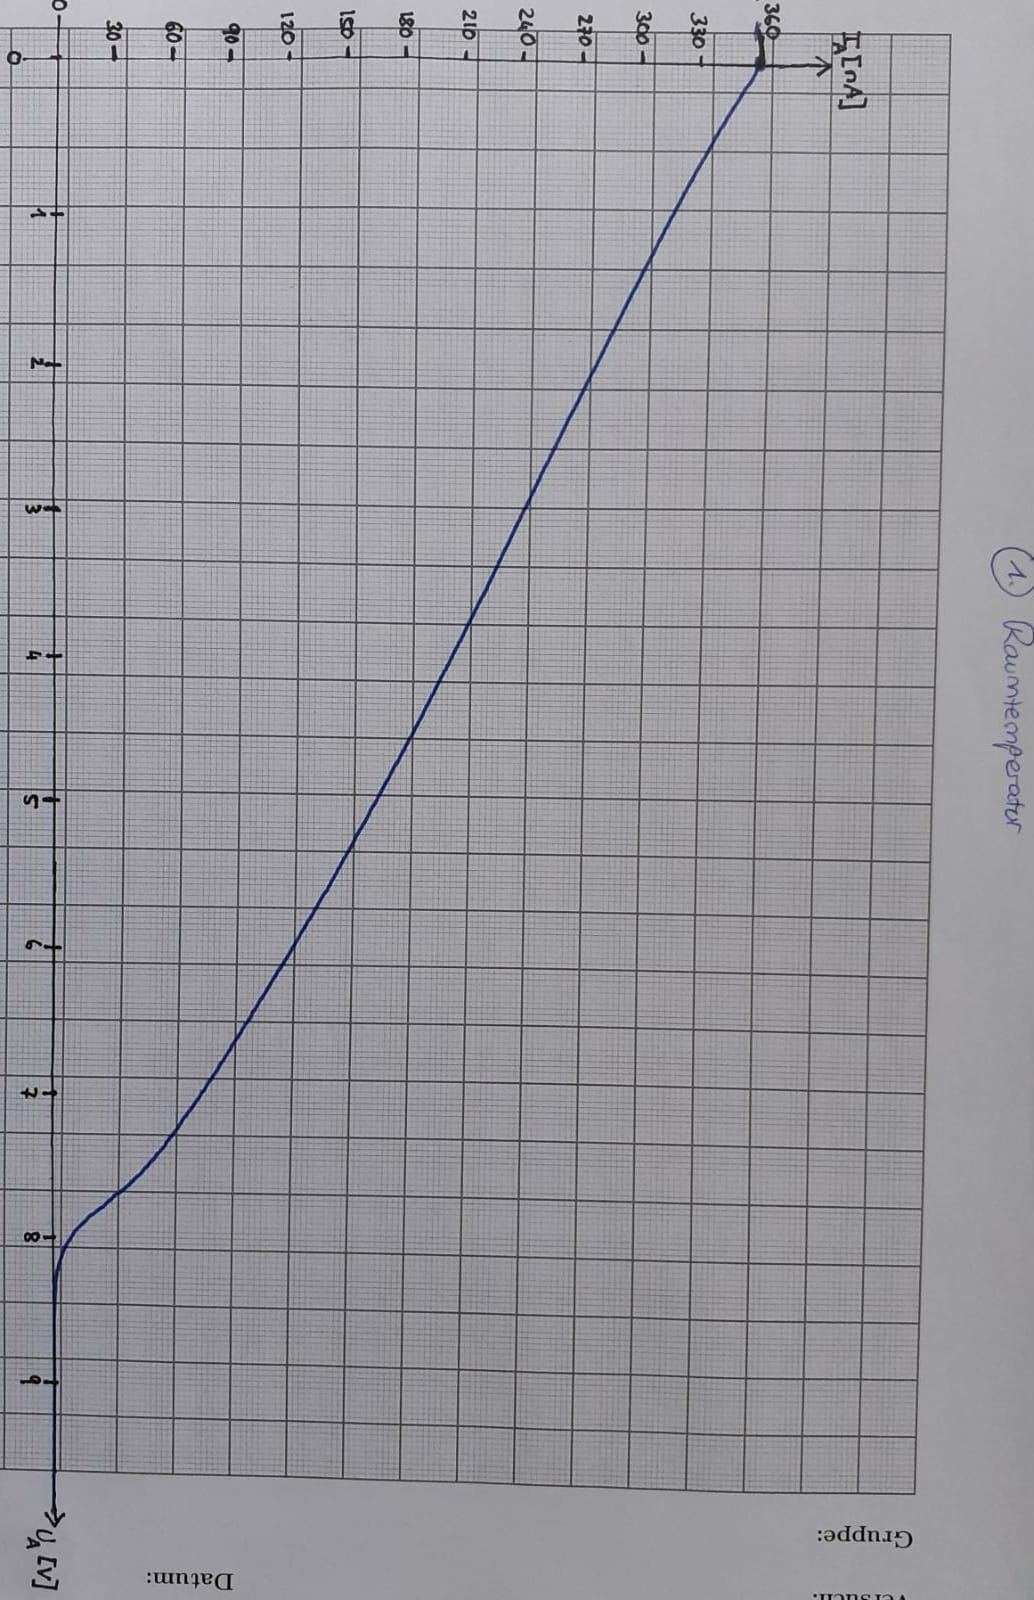
\includegraphics[width=0.6\textwidth,angle=90]{plots/Plot12.jpeg}
    \caption{Die vom XY-Schreiber aufgenommenen Messwerte zur integralen Energieverteilung der Elektronen.}
    \label{fig:EnergieMessFoto}
\end{figure}
\begin{figure}
    \centering
    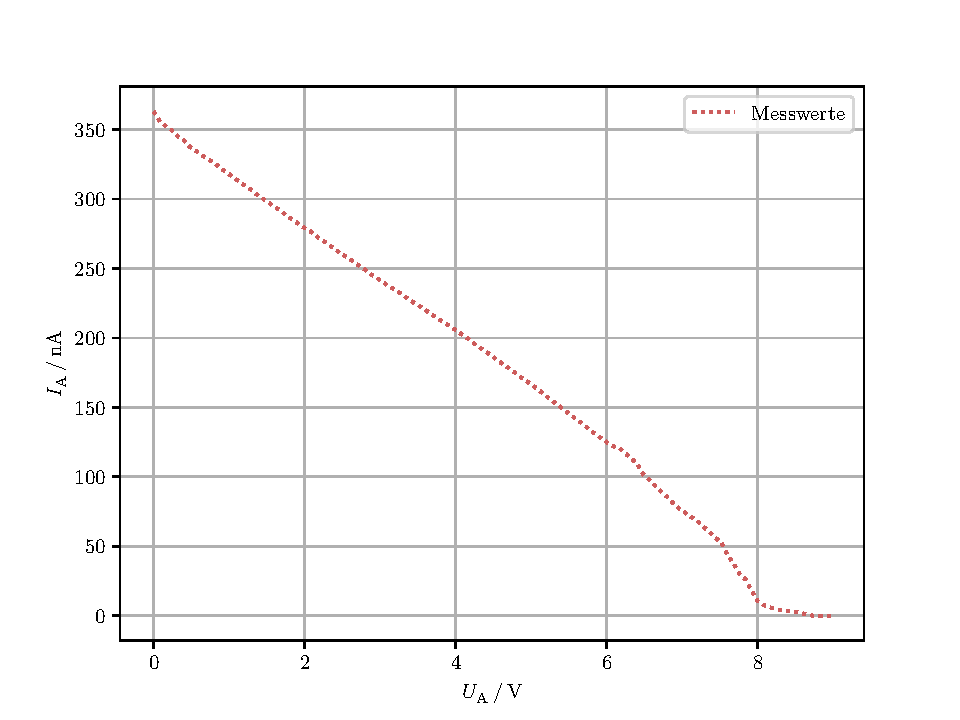
\includegraphics[width=\textwidth]{plots/Energie2.pdf}
    \caption{Die abgelesenen Messwerte zur integralen Energieverteilung der Elektronen.}
    \label{fig:EnergieMessAb}
\end{figure}

Um eine Aussage über die Energieverteilung der austretenden Elektronen machen zu können, muss die Differenz 
\begin{equation*}
    \Delta I_\text{A} := I_\text{A} (U) - I_\text{A} (U+\Delta U)
\end{equation*}
gebildet werden.

Der Strom $I_\text{A}$ ist proportional zur Anzahl $f(E)$ der ankommenden Elektronen und die Bremsspannung $U_\text{A}$ ist proportional zur Energie $E$ der Elektronen. 
Um die Verteilung der Elektronenzahl experimentell zu bestimmen, die eine Energie zwischen $E$ und $E+\symup{d}E$ haben, kann die Annäherung 
\begin{equation*}
    f(E)\,\symup{d}E \propto |\symup{d} I_\text{A}| = \left\vert\frac{\partial I_\text{A}}{\partial U_\text{A}}\right\vert \, \symup{d}U_\text{A} \approx \Delta I_\text{A} 
\end{equation*}
gemacht werden, sofern $\Delta U_\text{A} \ll U_\text{A}$ gilt. 
Hier wird aufgrund der Skalierung zwischen Kästchenzahl und Spannungswerten $\Delta U_\text{A} = \SI{0.08}{\volt}$ gewählt, wie aus den 
Tabellen \ref{tab:Energy1} und \ref{tab:Energy2} hervorgeht. 
Die entsprechende Graphik ist auf Abbildung \ref{fig:EnergieDiffAb} zu finden. 
\begin{figure}
    \centering
    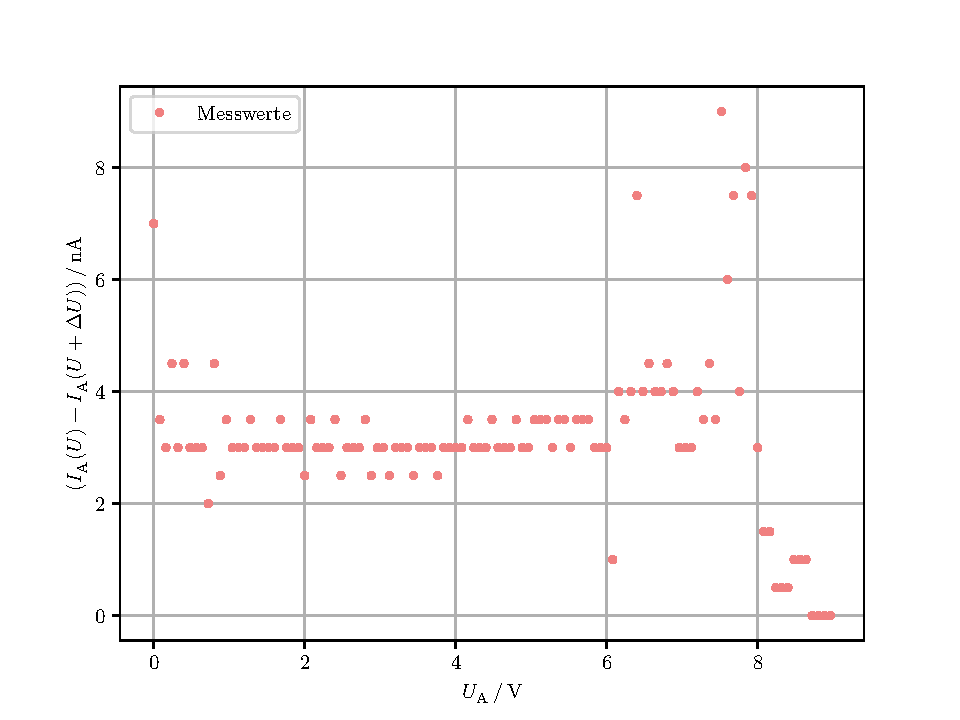
\includegraphics[width=\textwidth]{plots/EnergieDiff2.pdf}
    \caption{Die abgelesenen Messwerte zur differentiellen Energieverteilung der Elektronen.}
    \label{fig:EnergieDiffAb}
\end{figure}
Die Elektronen bekommen nach dem Austritt aus dem Glühdraht eine zusätzliche Energie von $\symup{e}U_\text{B}=\SI{11}{\electronvolt}$.
Mit großer Messunsicherheit lässt sich ein Maximum bei $\SI{7.7}{\volt}$ der ankommenden Elektronen feststellen. 
Daraus ergibt sich, dass die Elektronen ein zusätzliches Kontaktpotential von etwa
\begin{equation}
    K=(11-7.7)\,\si{\volt}=\SI{3.3}{\volt}
\end{equation}
überwinden müssen, wenn davon ausgegangen wird, dass die Stöße beim Durchqueren der Röhre die Messergebnisse nicht 
stark durch Richtungsablenkung verfälschen. 
Dafür spricht die vergleichsweise große mittlere freie Weglänge, die eine eher geringe Stoßwahrscheinlichkeit prognostiziert. 

Bei einer entsprechend höheren Temperatur wäre die Stoßwahrscheinlichkeit sehr viel größer, wie Tabelle \ref{tab:Weglänge} 
zu entnehmen ist. Wie stark die kinetische Energie in Richtung der Auffängerelektrode durch die Stöße verringert wird, 
ist zufällig. 
Ein Einbruch der Anzahl der ankommenden Elektronen würde bei erfolgreicher Messung da zu sehen sein, wo die Spannung abzüglich des Kontaktpotentials ausreicht, 
die Anregungsenergie der Hg-Atome aufzubringen. 

\subsection{Die Franck--Hertz-Kurve}

\begin{figure}
    \centering
    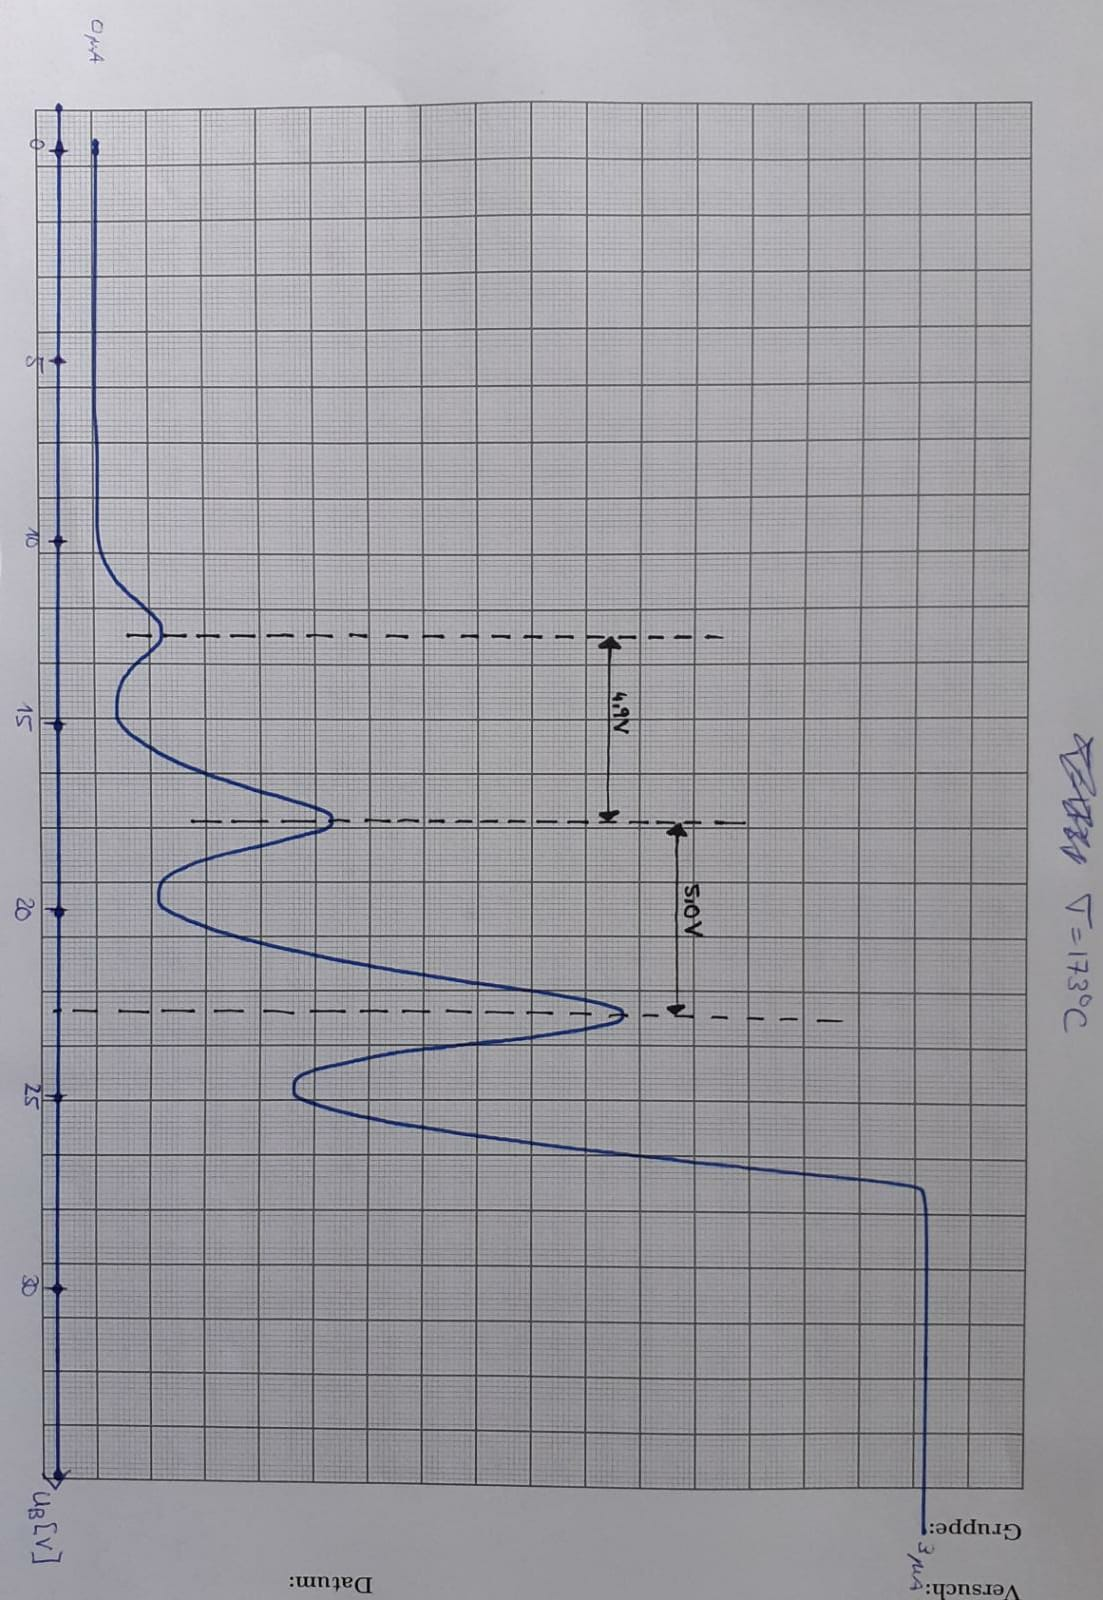
\includegraphics[width=0.6\textwidth,angle=90]{plots/Plot22.jpeg}
    \caption{Die vom XY-Schreiber aufgenommene Franck--Hertz-Kurve bei einer Temperatur von $\SI{173}{\degreeCelsius}$.}
    \label{fig:FrHeMess}
\end{figure}
In Abbildung \ref{fig:FrHeMess} ist die vom XY-Schreiber aufgenommene Franck--Hertz-Kurve zu sehen. 
Die Temperatur beträgt $\SI{173}{\degreeCelsius}$. 

Wie eingezeichnet lassen sich gut zwei Spannungsdifferenzen ablesen:
\begin{align*}
    \Delta U_1&=\SI{4.9}{\volt} \\
    \Delta U_2&=\SI{5.0}{\volt}
\end{align*}
Daraus ergibt sich unter Mittelwertbildung, Berechnung des Messfehlers mithilfe 
\begin{equation*}
    \bar{x}=\frac{1}{N}\sum_{i=1}^N x_i \quad \text{und}
\end{equation*}
\begin{equation*}
    \Delta x = \sqrt{\frac{1}{N-1} \sum_{i=1}^N (x_i-\bar{x})^2}
\end{equation*}
und Runden auf die signifikanten Ziffern eine Anregungsenergie von 
\begin{equation}
    \Delta E_\text{exp}=\symup{e}\cdot \Delta U = \SI{5.0+-0.1}{\electronvolt}\,.
\end{equation}
Da das Kontaktpotential ausschließlich eine Verschiebung der Strommaxima bewirkt und für das Berechnen der 
Anregungsenergie ausschließlich die Spannungsdifferenzen relevant sind, muss das Kontaktpotential nicht beachtet werden. 

Die weiteren elastischen Stöße, die die Elektronen nach einem (oder ein paar wenigen mehr) inelastischen Stößen ausführen, 
werden nicht beachtet, unter der Annahme, dass dies am Verhältnis der ankommenden und nicht-ankommenden Elektronen an der 
Auffängerelektrode nichts verändern wird. 

$\Delta E_\text{exp}$ entspricht mit $E=\symup{h}\sfrac{\symup{c}}{\lambda}$ (das Planck'sche Wirkungsquantum ist laut \cite{scipy}
$\symup{h}=\SI{4.135667662e-15}{\electronvolt\second}$ und die Lichtgeschwindigkeit im Vakuum ist $\symup{c}=\SI{299792458.0}{\meter\per\second}$)
elektromagnetischer Strahlung der Wellenlänge 
\begin{equation}
    \lambda _\text{exp}=\SI{248+-5}{\nano\meter}\,,
\end{equation}
die somit kurzwelliger als ultraviolettes Licht ist.

%Das erste Strommaxima unter Vernachlässigung der Abflachung der Peaks (vgl. Kapitel \ref{sec:Theorie}) liegt bei etwa $(5-3.3)\,\si{\volt}=\SI{1.7}{\volt}$, was 
%aufgrund der Skalierung des Picoamperemeters jedoch nicht zu überprüfen ist. 
